\begin{spacing}{1.15}
\pagestyle{plain}

% =========================================================================
% APPENDIX A: PROJECT TIMELINE
% =========================================================================
\clearpage
\thispagestyle{plain}
\pagestyle{plain}
\addcontentsline{toc}{chapter}{APPENDIX A: PROJECT TIMELINE}
\markboth{}{}
\renewcommand{\thefigure}{A.\arabic{figure}}
\setcounter{figure}{0}
\renewcommand{\thetable}{A.\arabic{table}}
\setcounter{table}{0}
\renewcommand{\theequation}{A.\arabic{equation}}
\setcounter{equation}{0}

\vspace*{-0.5cm}

\begin{center}
{\Large \textbf{APPENDIX A\\[0.35em] PROJECT TIMELINE}}\par
\end{center}

\vspace{0.3cm}

\begin{table}[H]
\centering
\caption{Comprehensive Project Timeline and Development Milestones Summary}
\label{tab:dev_timeline}
\vspace{0.25cm}
\setlength{\tabcolsep}{4pt}
\renewcommand{\arraystretch}{1.20}
\begin{tabular}{|>{\raggedright\arraybackslash}p{0.24\textwidth}|>{\centering\arraybackslash}p{0.15\textwidth}|>{\raggedright\arraybackslash}p{0.36\textwidth}|>{\raggedright\arraybackslash}p{0.16\textwidth}|}
\hline
\textbf{Phase / Milestone} & \textbf{Period / Date} & \textbf{Development Work Done \& Progress Status} & \textbf{Evaluation / Marks} \\ \hline
\textbf{Phase 1: Inception \& Project Proposal} (Weeks 1--4) & 02.07.2026 -- 31.07.2026 & Topic finalized with guide Dr.~Indu John; literature review completed; SRS prepared; zero-hardware webcam architecture defined. & Topic Approval (Preliminary) \\ \hline
\textbf{Phase 2: Baseline Model \& Interim Review} (Weeks 5--7) & 03.08.2026 -- 28.08.2026 & MediaPipe Holistic pipeline built; 2D/3D normalization implemented; baseline classifier trained; $\sim$20\% prototype approved. & Interim Review 1 (20 Marks) \\ \hline
\textbf{Phase 3: Core Engine \& Web Interface} (Weeks 8--11) & 31.08.2026 -- 25.09.2026 & Web interface built (HTML5/CSS3/JS); open-set rejection ($\tau = 0.35$) tuned; sentence builder and speech synthesis integrated; $\sim$50\% demo verified. & Interim Review 2 (20 Marks) \\ \hline
\textbf{Phase 4: Web Studios \& Retraining Engine} (Weeks 12--14) & 28.09.2026 -- 16.10.2026 & Interactive AI Retraining Studio built with validation gate; Practice Studio developed with HUD score; latency profiled at 18.4 ms. & Progress Review (Completed) \\ \hline
\textbf{Phase 5: Final Review \& Documentation} (Weeks 15--17) & 19.10.2026 -- 06.11.2026 & Phase I 80\% milestone achieved; report formatted; IJERA manuscript submitted; live demo delivered; Phase II roadmap defined. & Final Review (50 Marks: 10+10+30) \\ \hline
\end{tabular}
\end{table}

% =========================================================================
% APPENDIX B: SCREENSHOTS
% =========================================================================
\clearpage
\chapter*{APPENDIX B \\ SCREENSHOTS}
\pagestyle{plain}
\thispagestyle{plain}
\addcontentsline{toc}{chapter}{APPENDIX B: SCREENSHOTS}
\markboth{}{}
\renewcommand{\thefigure}{B.\arabic{figure}}
\setcounter{figure}{0}
\renewcommand{\thetable}{B.\arabic{table}}
\setcounter{table}{0}
\renewcommand{\theequation}{B.\arabic{equation}}
\setcounter{equation}{0}

\begin{singlespace}
\noindent The ISL-Lens web-native platform provides a unified, responsive graphical user interface designed for frictionless accessibility across standard personal computers and laptops. This appendix presents authentic interface screenshots corresponding to the three primary operational subsystems:

\begin{enumerate}
    \setlength{\itemsep}{2pt}
    \item \textbf{Main Recognition Console}: Displays the primary web-native dashboard comprising the live recognition viewport, real-time status badges, Meet-style dock controls, continuous sentence generation panel, conversation transcript log, and the interactive vocabulary dictionary (Figure \ref{fig:app_console}).
    \item \textbf{Interactive Sign Practice Studio}: Features a dual-viewport comparison layout for sign rehearsal against verified dataset demonstration videos, real-time match percentage feedback, and structured kinetic guidance (Figure \ref{fig:app_practice}).
    \item \textbf{Interactive AI Retraining Studio}: Presents the unified gesture recording interface for on-device personalized sign acquisition and automated model update validation (Figure \ref{fig:app_studio}).
\end{enumerate}

\begin{figure}[H]
\centering
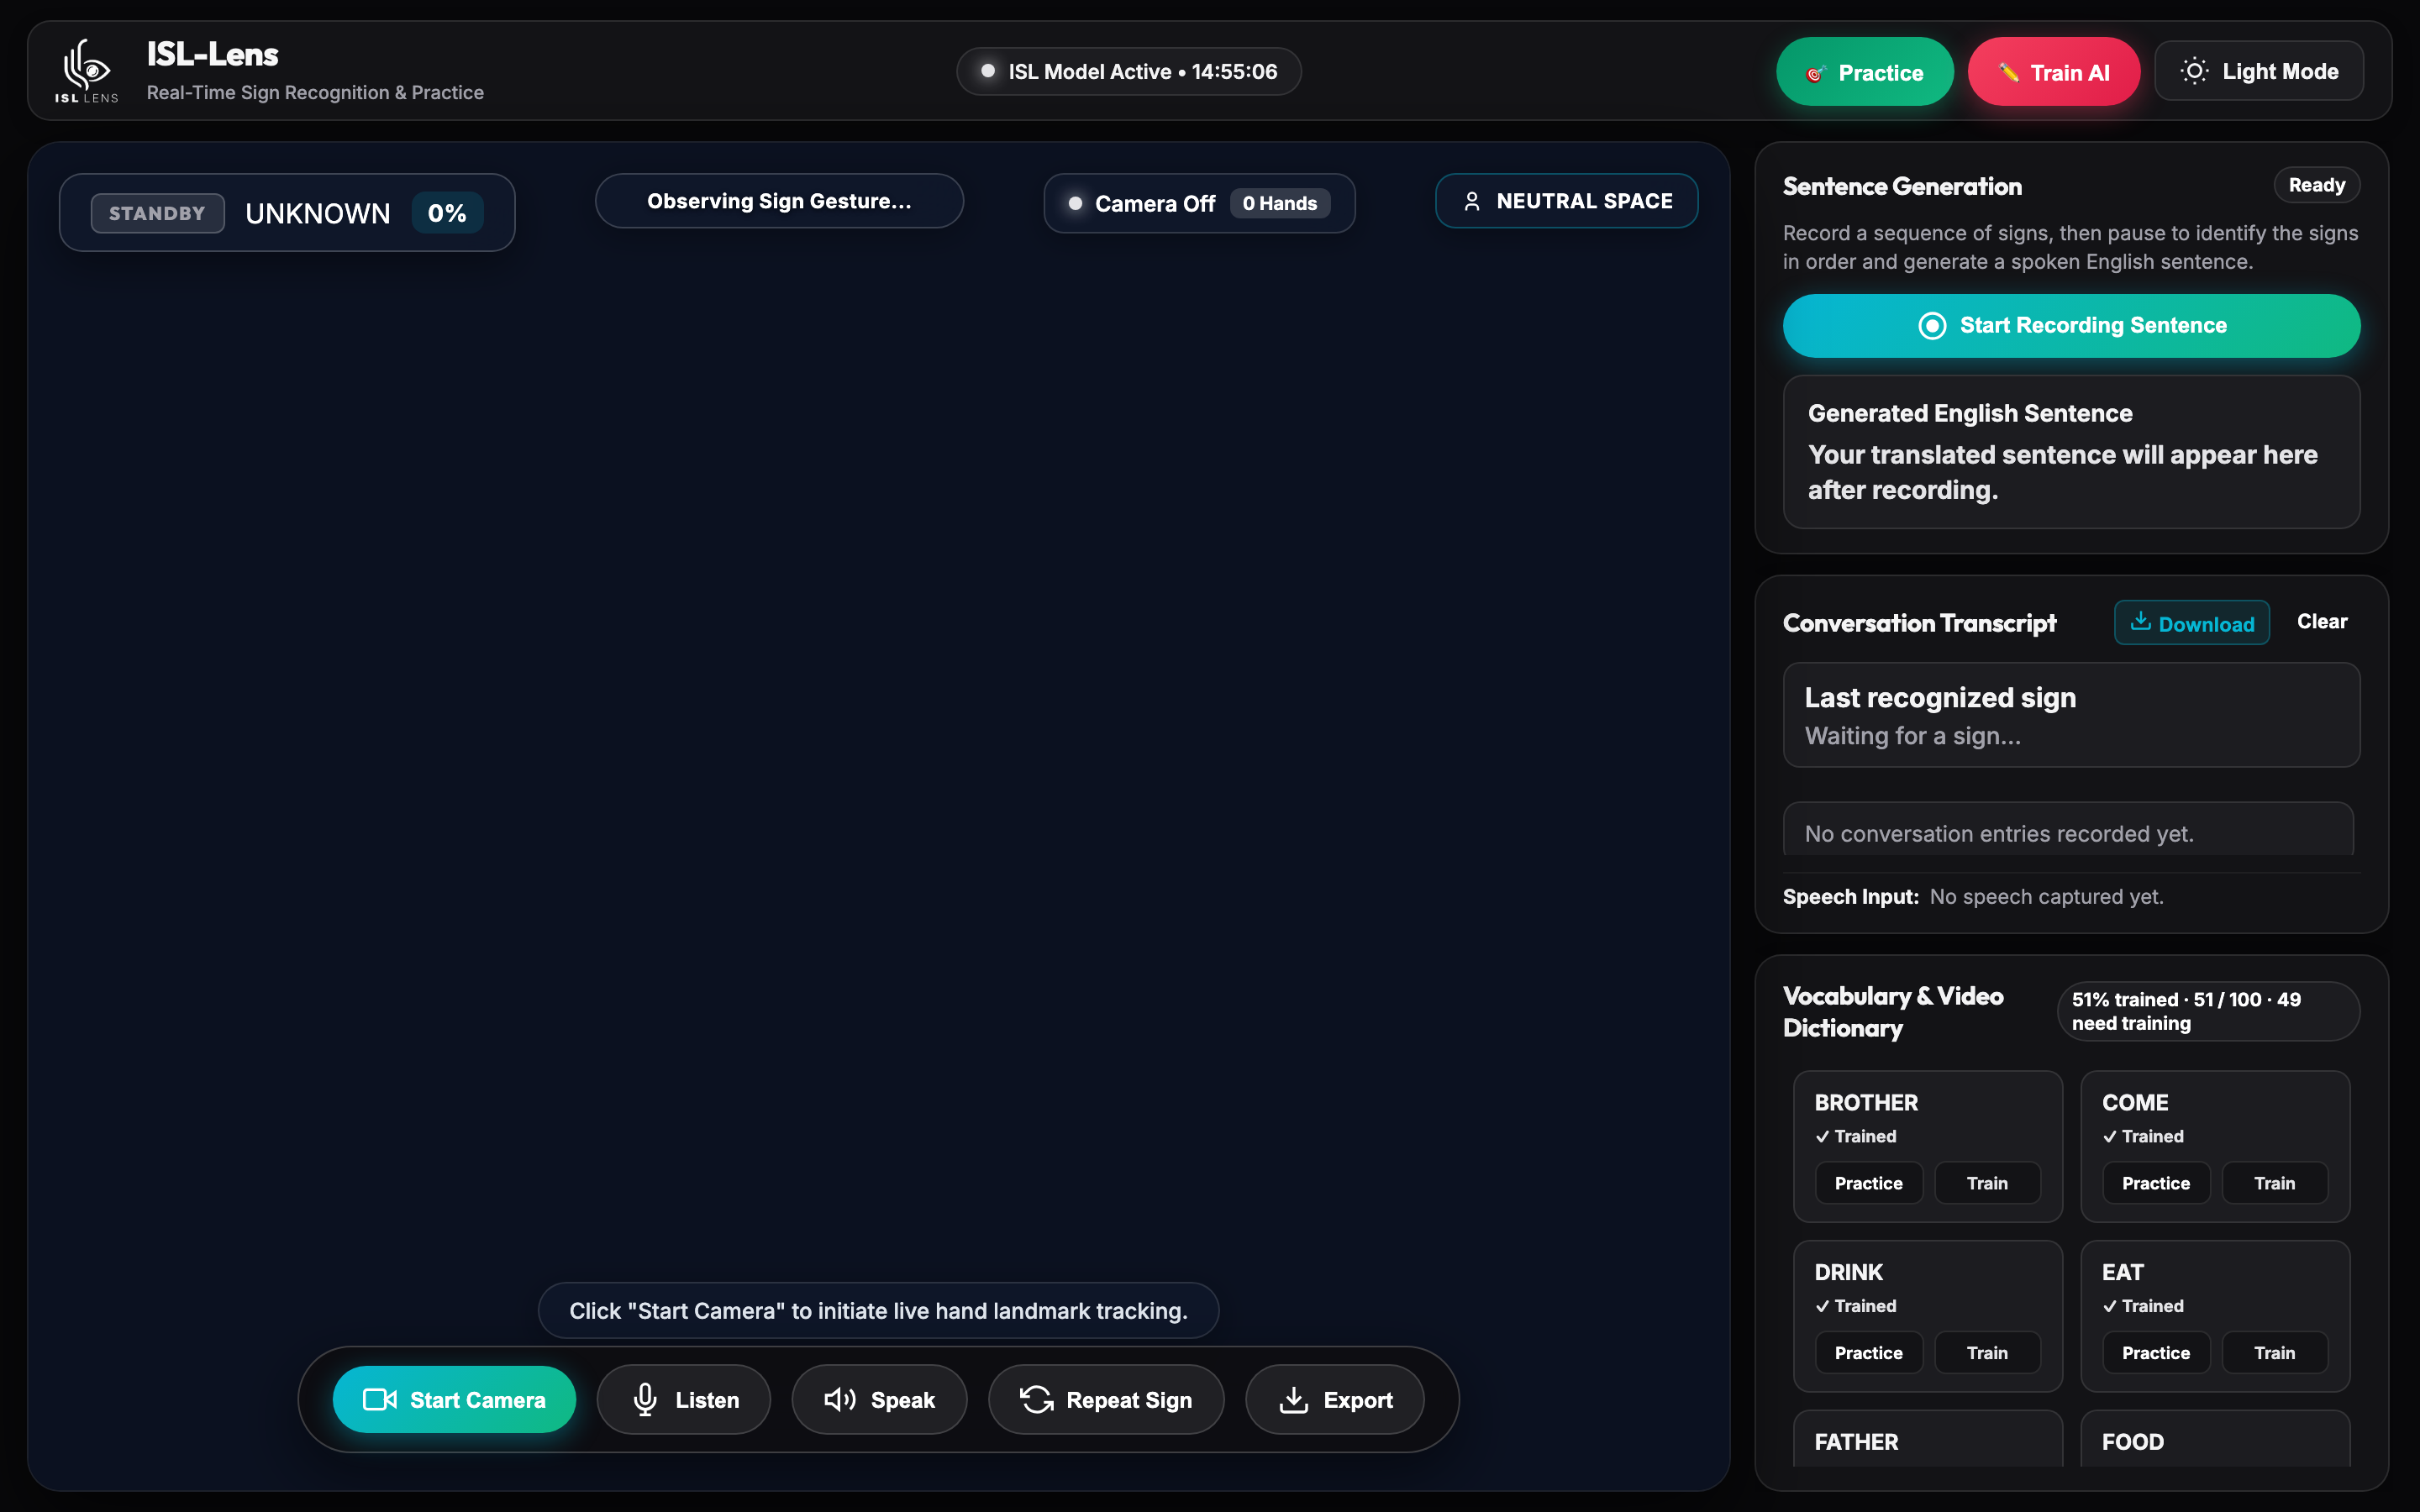
\includegraphics[width=0.68\textwidth]{fig_browser_console.png}
\caption{Main User Interface of the ISL-Lens Real-Time Recognition Console.}
\label{fig:app_console}
\end{figure}
\end{singlespace}

\clearpage
\thispagestyle{plain}

\begin{figure}[H]
\centering
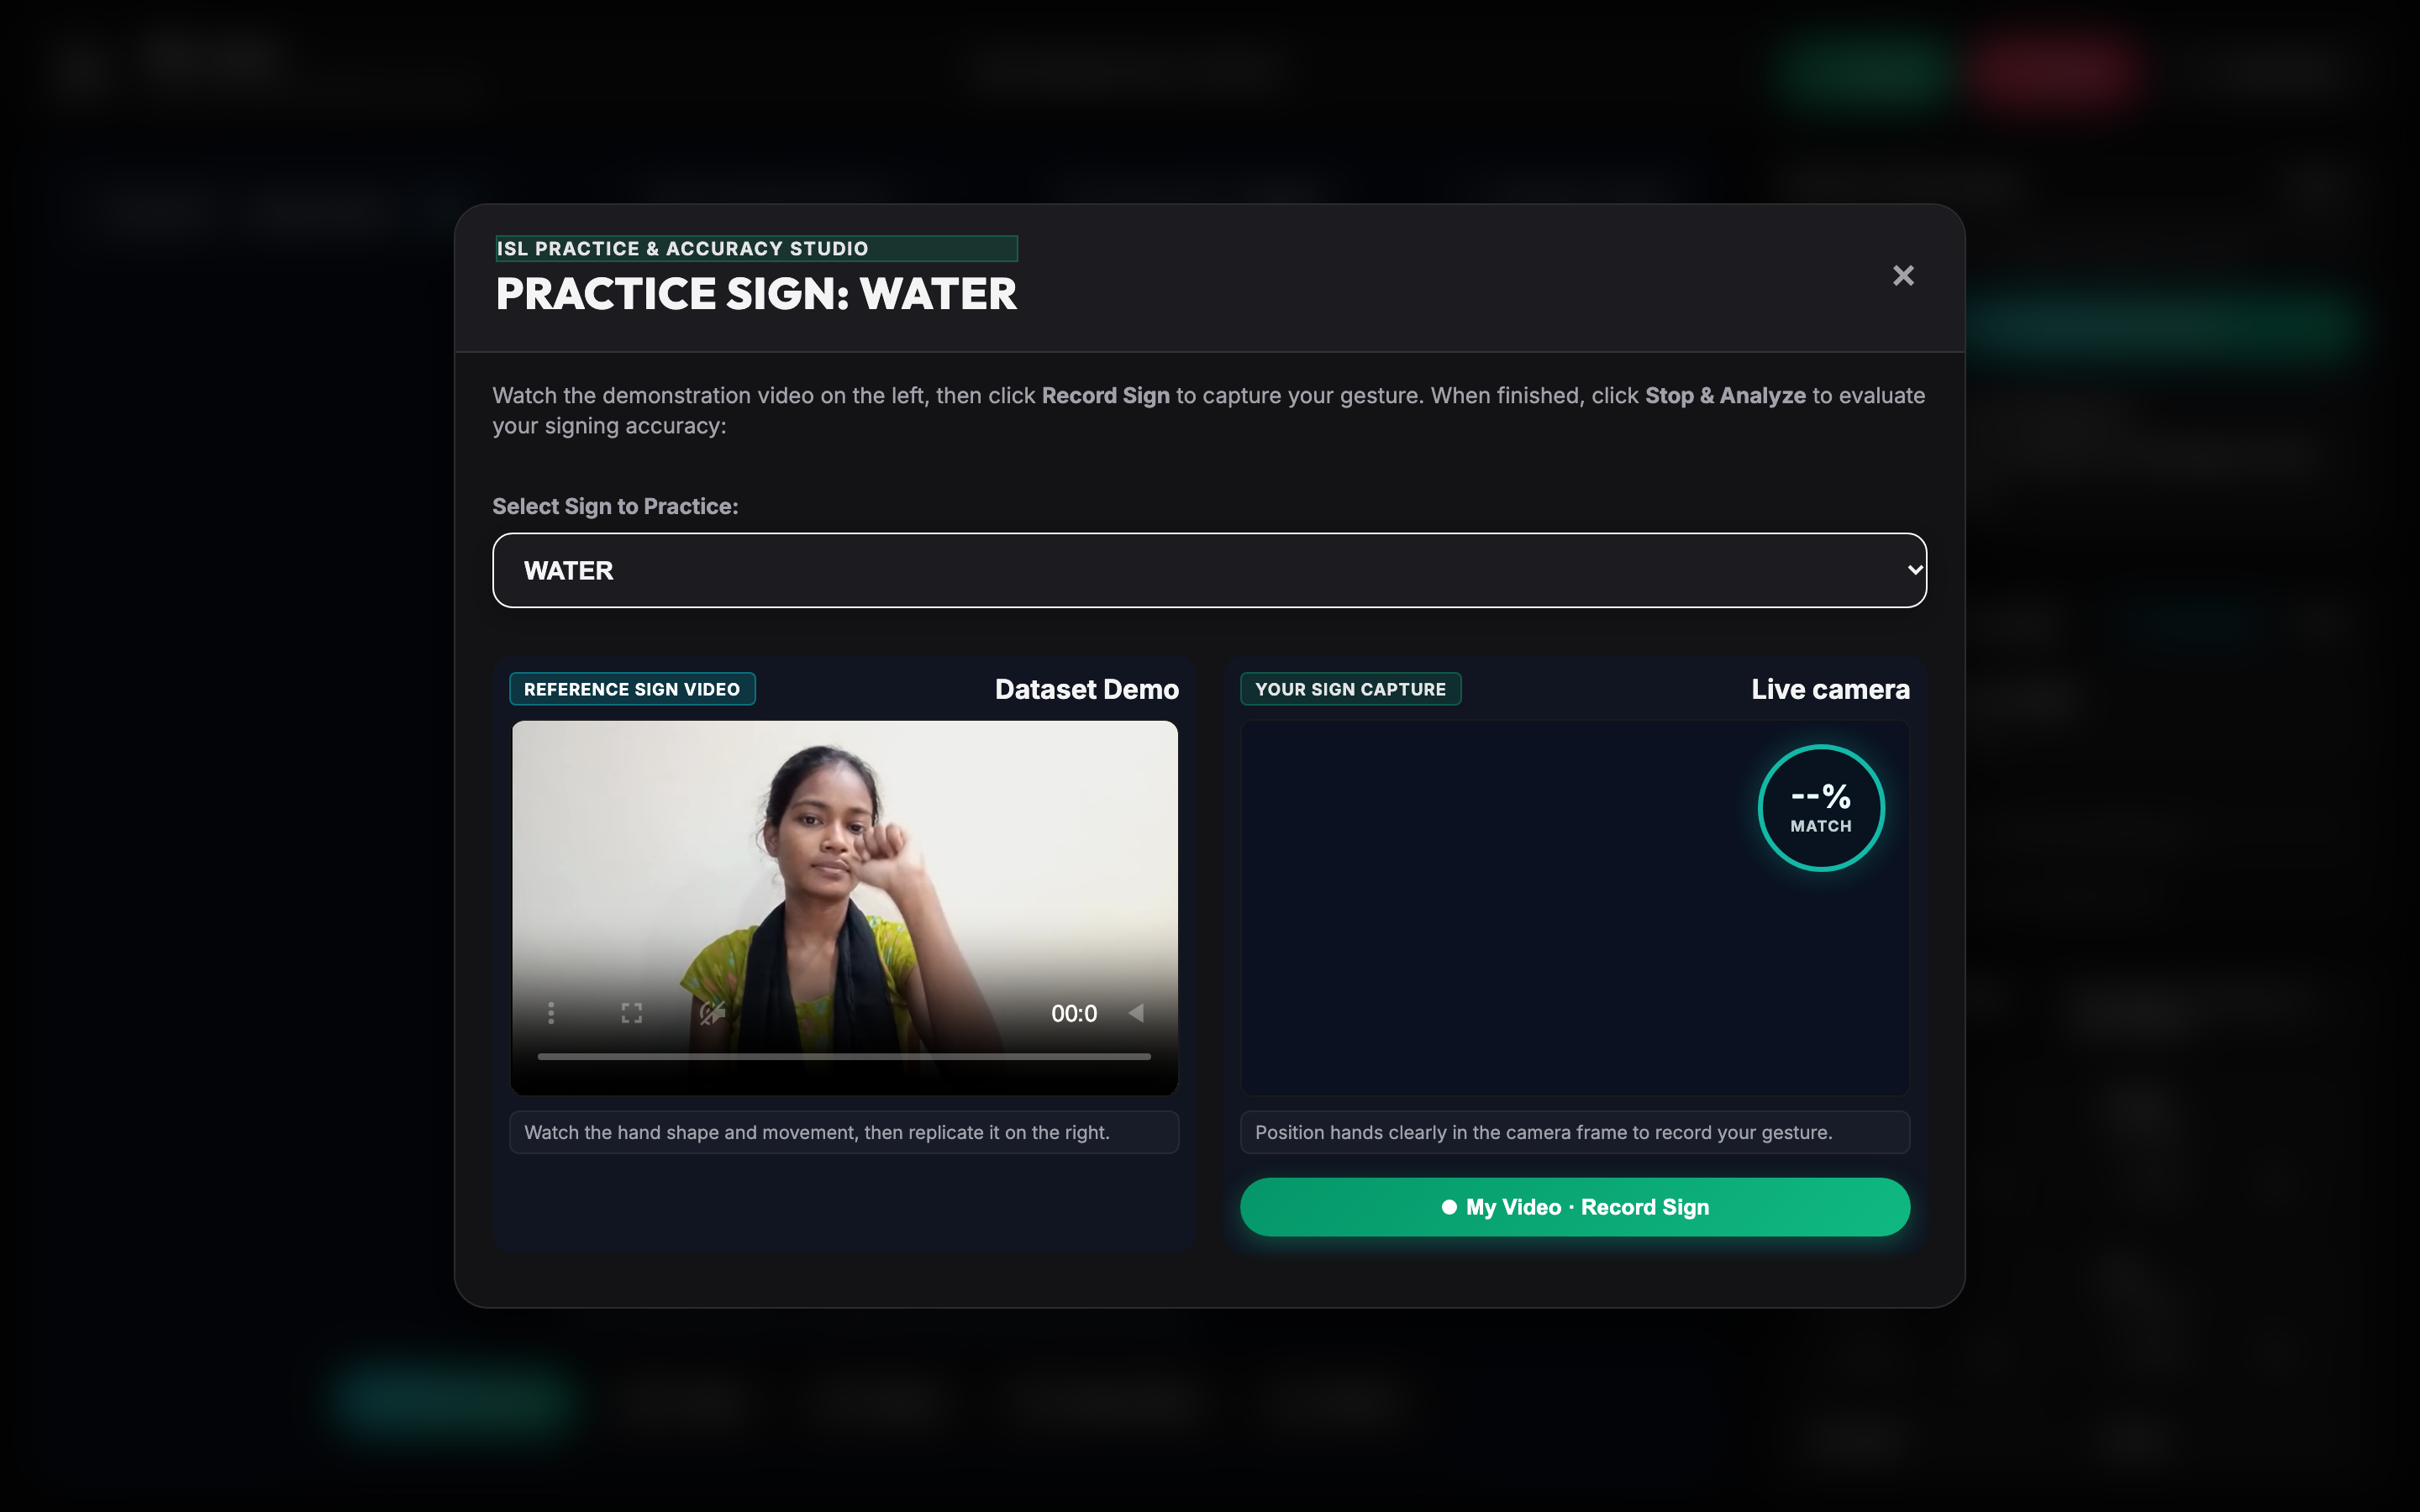
\includegraphics[width=0.71\textwidth]{fig_browser_practice.png}
\caption{Interactive Sign Practice Studio Interface with Reference Demonstration for WATER.}
\label{fig:app_practice}
\vspace{0.4cm}
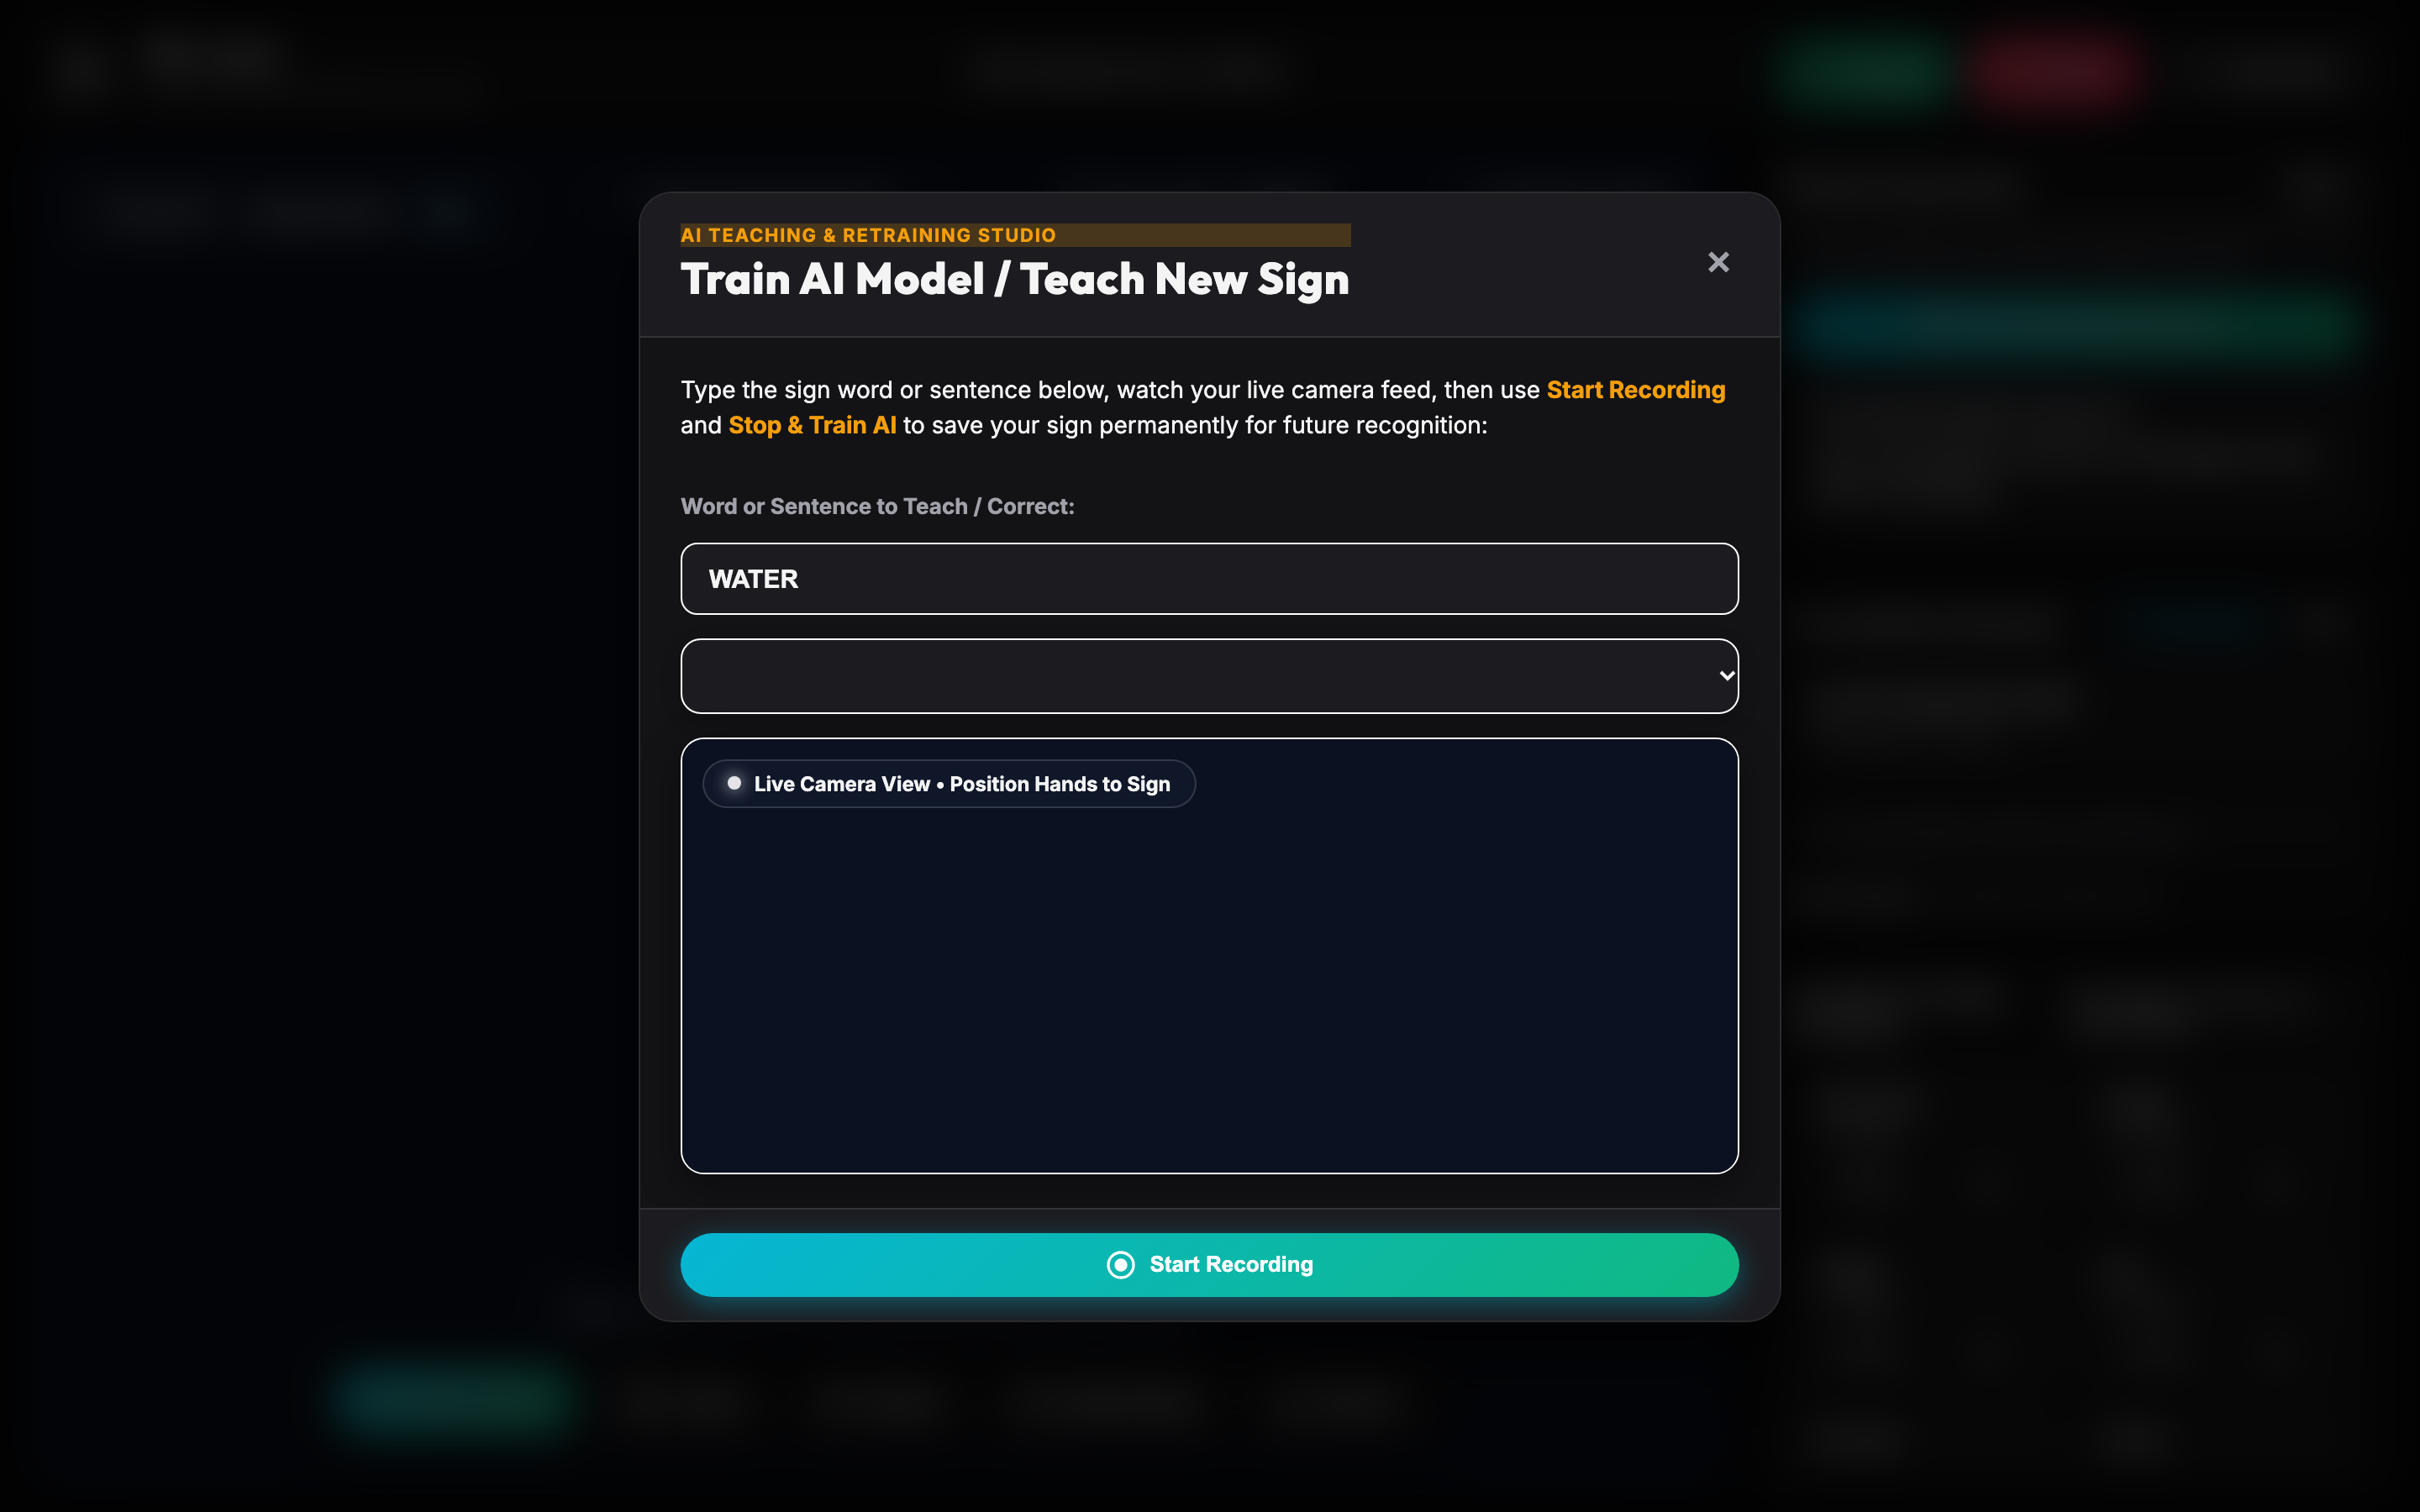
\includegraphics[width=0.71\textwidth]{fig_browser_studio.png}
\caption{Interactive AI Retraining and Model Fine-Tuning Studio Interface.}
\label{fig:app_studio}
\end{figure}

% =========================================================================
% APPENDIX C: PUBLICATION
% =========================================================================
\clearpage
\chapter*{APPENDIX C \\ PUBLICATION}
\pagestyle{plain}
\thispagestyle{plain}
\addcontentsline{toc}{chapter}{APPENDIX C: PUBLICATION}
\markboth{}{}
\renewcommand{\thefigure}{C.\arabic{figure}}
\setcounter{figure}{0}
\renewcommand{\thetable}{C.\arabic{table}}
\setcounter{table}{0}
\renewcommand{\theequation}{C.\arabic{equation}}
\setcounter{equation}{0}

\section*{Journal Paper Submission Details}

\noindent Based on the research findings and architecture formulated during Phase I of this B.Tech project, an original research manuscript was authored and submitted for peer-reviewed publication to the \textbf{International Journal on Emerging Research Areas (IJERA)}:

\begin{table}[H]
\centering
\caption{Publication Submission Specifications for IJERA Manuscript}
\label{tab:ijera_specifications}
\vspace{0.2cm}
\renewcommand{\arraystretch}{1.25}
\begin{tabular}{|>{\raggedright\arraybackslash}p{0.32\textwidth}|>{\raggedright\arraybackslash}p{0.62\textwidth}|}
\hline
\textbf{Parameter} & \textbf{Submission Specification} \\ \hline
\textbf{Paper Title} & \textit{ISL-LENS: Real-Time Indian Sign Language Recognition And Interactive AI Console} \\ \hline
\textbf{Author} & Aevlin Prince (\texttt{aevlinprince2027@cs.ajce.in}) \\ \hline
\textbf{Academic Department} & Department of Computer Science and Engineering \\ \hline
\textbf{Institution} & Amal Jyothi College of Engineering (Autonomous), Kanjirappally \\ \hline
\textbf{Target Journal} & International Journal on Emerging Research Areas (IJERA) \\ \hline
\textbf{Editorial Communication} & Dr.~Juby Mathew, Editor \& HoD CSE (\texttt{ijera@amaljyothi.ac.in}) \\ \hline
\textbf{Submission ID / No.} & 554 \\ \hline
\textbf{Tracking Dashboard URL} & \url{https://ijera.in/index.php/IJERA/authorDashboard/submission/554} \\ \hline
\textbf{Submission Timestamp} & 26 October 2026 at 08:29 AM IST \\ \hline
\textbf{Current Status} & Under Editorial Peer Review \\ \hline
\end{tabular}
\end{table}

\clearpage
\thispagestyle{plain}

\vspace*{1.8cm}

\begin{figure}[H]
\centering

\includegraphics[width=0.88\textwidth,height=0.72\textheight,keepaspectratio]{fig_ijera_submission_mail.png}
\vspace{0.3cm}
\caption{Official journal submission acknowledgment letter from IJERA for Paper ID 554.}
\label{fig:ijera_acknowledgment}
\end{figure}

\end{spacing}
